\chapter{Experimental Evaluation}
\label{ch:experiments}

In Fig.~\ref{fig:figure_1}~(a) -- (d) some very nice figures are shown. In this figure the possibility of displaying subfigures is used. The width of each subfigure is fixed via parameter \texttt{width}. Note that parameter \texttt{[h]} is \textit{not} recommended at all -- most of the time \LaTeX~knows very well where a figure should be placed -- use the parameter only if there is really no other way. 

\begin{figure}[h] % do NOT use parameter h!
\centerline{
\subfigure[Title]{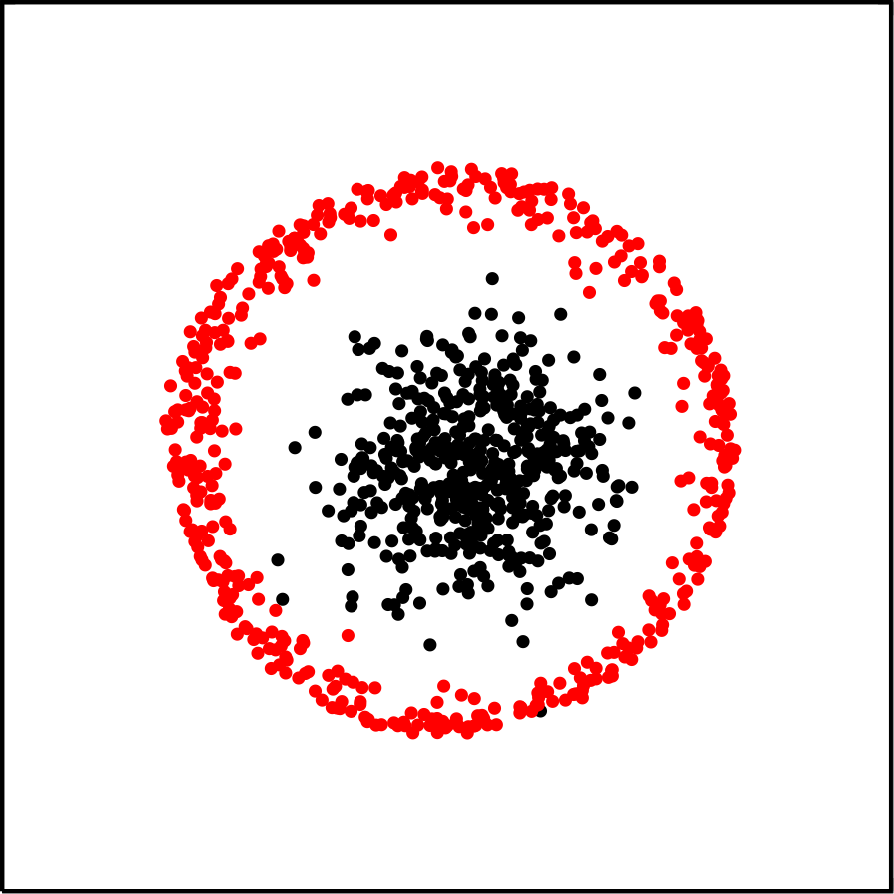
\includegraphics[width=1.5in]{img/subfig_a}}
\subfigure[Title]{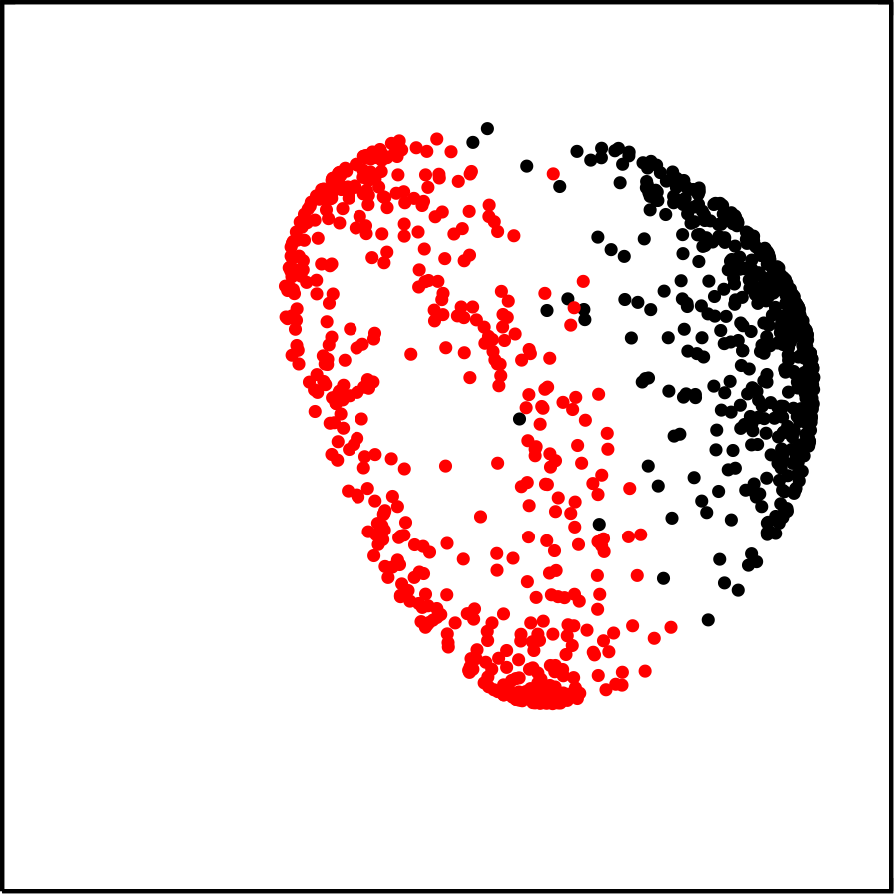
\includegraphics[width=1.5in]{img/subfig_b}}
}
\centerline{
\subfigure[Title]{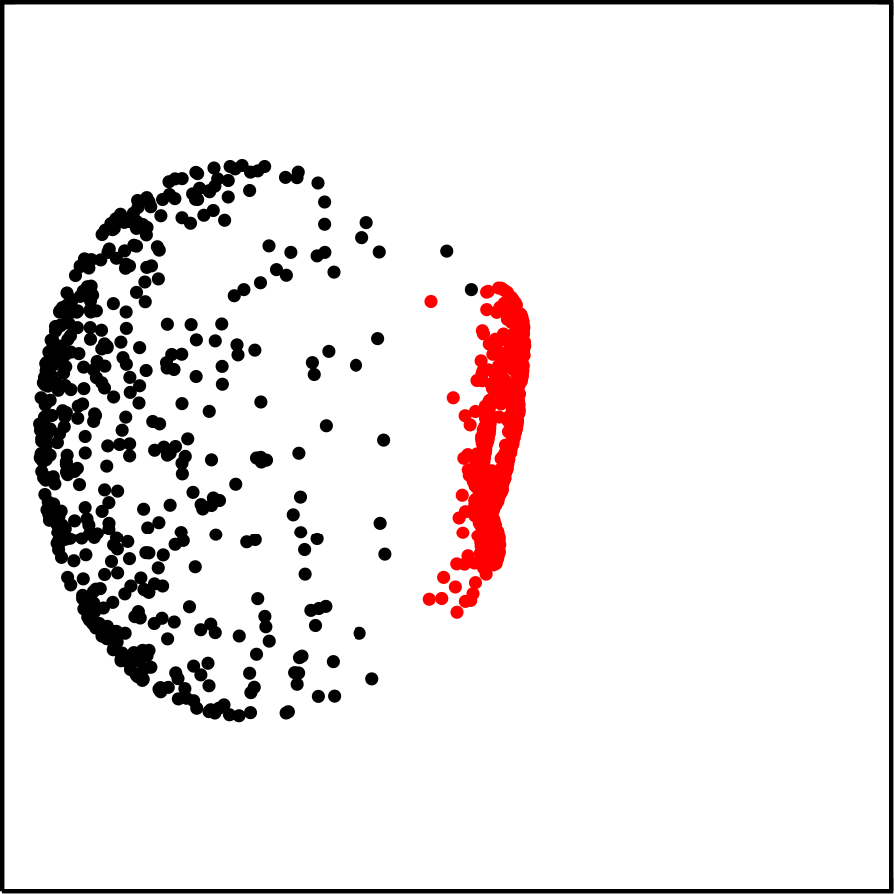
\includegraphics[width=1.5in]{img/subfig_c}}
\subfigure[Title]{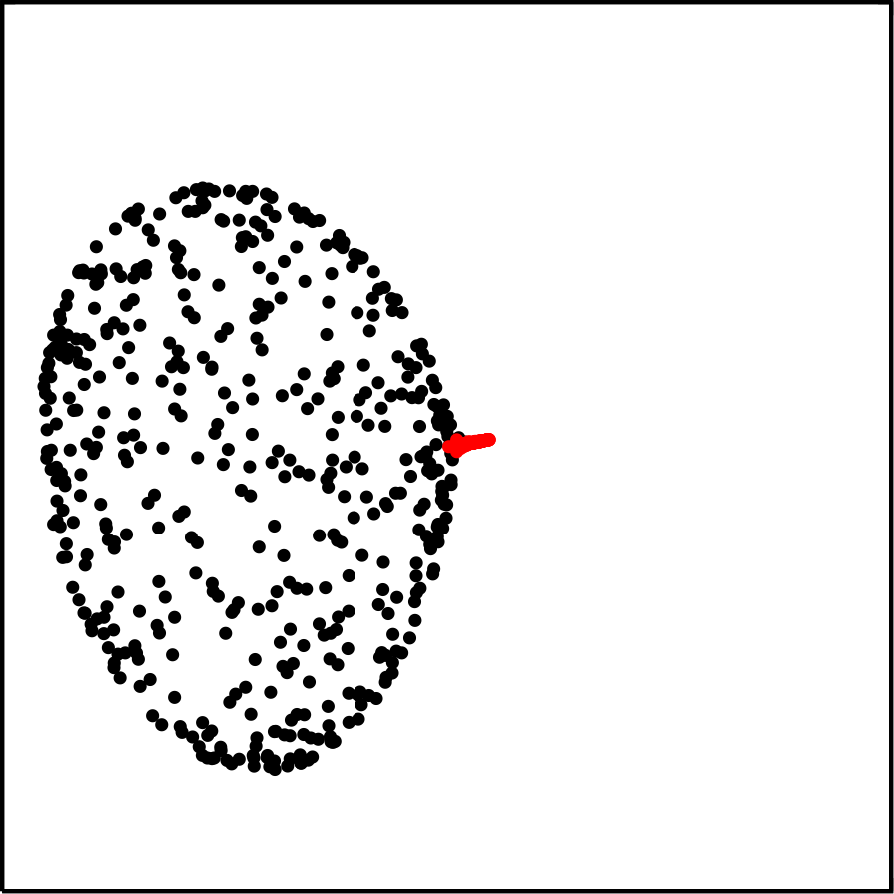
\includegraphics[width=1.5in]{img/subfig_d}}
}

\caption{Caption of the complete figure.}
\label{fig:figure_1}
\end{figure} 	


In Fig.~\ref{fig:figure_2} the \textit{Lorem ipsum} is illustrated. This time a single figure (without subfigures) is shown. Note how parameter \texttt{scale} rather than \texttt{width} is employed to manage the size of this figure.


\begin{figure}
\centering
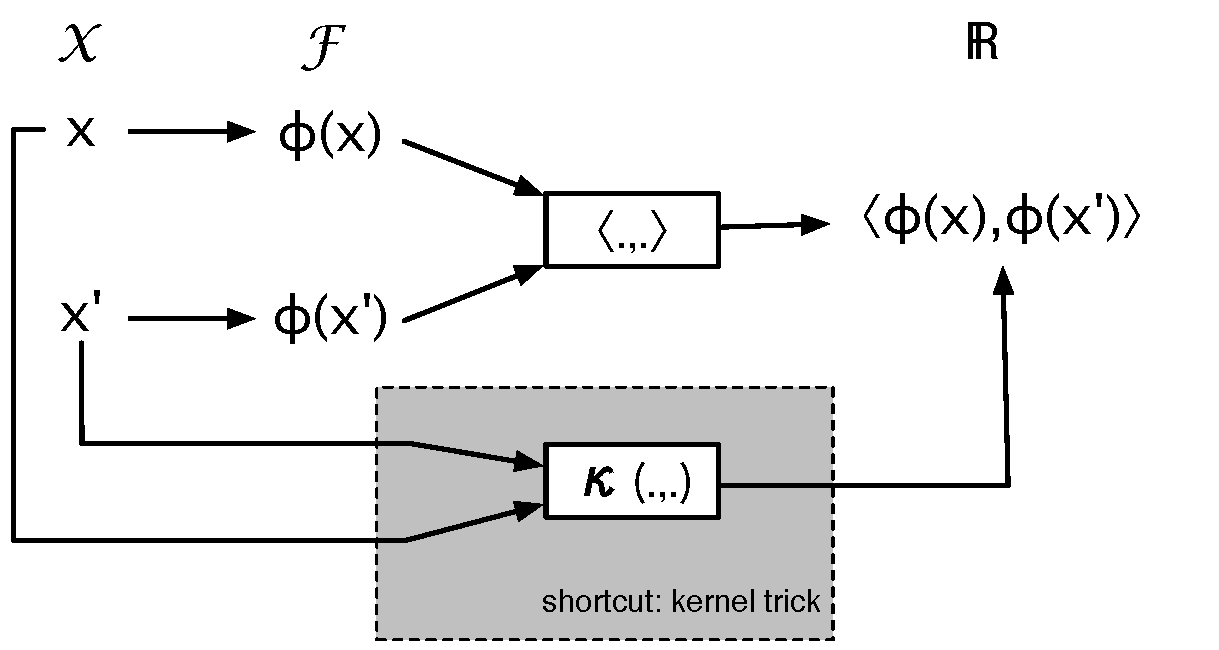
\includegraphics[scale=0.5]{img/figure}
\caption{Caption of this figure.}
\label{fig:figure_2}
\end{figure}



In Table~\ref{tab:table_1} some basic characteristics of consetetur sadipscing are shown in a rather simple format. Table~\ref{tab:table_2} is more elaborated and uses, for instance, multicolumns and other features.


\begin{table}
\centering
{
\begin{tabular}{ll}
\addlinespace
\toprule
\addlinespace
Lorem Ipsum \\
\addlinespace
\toprule
\addlinespace
diam & vero eos et accusam et justo \\
justo & 10 (0, 1, 2, 3, 4, 5, 6, 7, 8, 9) \\
aliquyam (q, w, t) &1,000, 500, 2,000\\
voluptua & nonumy eirmod tempor (takimata sanctus)\\
tempor & none \\
gubergren & yes \\
\bottomrule
\end{tabular}
}
\caption{Basic characteristics of Lorem Ipsum.}
\label{tab:table_1} 
\end{table}




\begin{table}
\footnotesize{
\centering{
\begin{tabular}{@{}lp{1cm}p{1cm}p{1cm}p{1cm}@{}}
\addlinespace
\toprule
\addlinespace
& $k$-ta & \multicolumn{2}{c}{Lorem Ipsum Dolor}\\ 
\addlinespace
Ea Rebum & te & va & te\\ 
\addlinespace
\hline
\addlinespace
Gubergren           & 94.9 & 98.0 & 97.0~\ding{172}  \\
\addlinespace
Magna   & 66.9 & 72.4 & 68.6~\ding{182}  \\
\addlinespace
\bottomrule
\end{tabular}
}
\caption{Lorem ipsum dolor sit amet, consetetur sadipscing elitr, sed diam nonumy eirmod tempor invidunt ut labore et dolore magna aliquyam erat, sed diam voluptua ($\alpha=0.05$): \ding{172}/\ding{182} At vero eos et accusam/justo, respectively.}
\label{tab:table_2}
}
\end{table}



